%%%%%%%%%%%%%%%%%%%% author.tex %%%%%%%%%%%%%%%%%%%%%%%%%%%%%%%%%%%
%
% sample root file for your "contribution" to a proceedings volume
%
% Use this file as a template for your own input.
%
%%%%%%%%%%%%%%%% Springer %%%%%%%%%%%%%%%%%%%%%%%%%%%%%%%%%%


\documentclass{svproc}
\usepackage{marvosym}

%%%%%%%%%%%%%%%%%%%%%%%%%%%%%%%%%%%%%%%%%%%%%%%%%%%%%%%%%%%%%%%%%%%
% Для русского яыка. потом надо убрать
% % \usepackage[unicode]{hyperref}
% % \usepackage[utf8x]{inputenc}
% \usepackage[T1,T2A]{fontenc}
% \usepackage[utf8]{inputenc}
% \usepackage[english,russian]{babel}
% \DeclareUnicodeCharacter{0306}{}

%%%%%%%%%%%%%%%%%%%%%%%%%%%%%%%%%%%%%%%%%%%%%%%%%%%%%%%%%%%%%%%%%%%
% Columns: https://www.overleaf.com/learn/latex/Multiple_columns
% \usepackage{blindtext}
% \usepackage{multicol}
% \setlength{\columnsep}{1cm}

%%%%%%%%%%%%%%%%%%%%%%%%%%%%%%%%%%%%%%%%%%%%%%%%%%%%%%%%%%%%%%%%%%%











% RECOMMENDED
\usepackage{graphicx}

% to typeset URLs, URIs, and DOIs
\usepackage{url}
\usepackage{hyperref}
\def\UrlFont{\rmfamily}
\providecommand{\doi}[1]{doi:\discretionary{}{}{}#1}

\def\orcidID#1{\unskip$^{[#1]}$}
\def\letter{$^{\textrm{(\Letter)}}$}










\begin{document}
\mainmatter % start of a contribution

\title{A New Version of the AlgoView System for 3D Visualization and Interactive Analysis of Information Graphs of Algorithms}

\titlerunning{A New Version of the AlgoView}  % abbreviated title (for running head)
                                              % also used for the TOC unless
                                              % \toctitle is used

% \orcidID{0000-1111-2222-3333}
\author{Gleb Skryabin\inst{1, 2}\letter \and Tamara Gadieva\inst{1, 2} \and Alexander Antonov\inst{2}}

\authorrunning{G. Skryabin, T. Gadieva, A. Antonov} % abbreviated author list (for running head)

%%%% list of authors for the TOC (use if author list has to be modified)
\tocauthor{Gleb Skryabin and Tamara Gadieva, and Alexander Antonov}

\institute{Lomonosov Moscow State University \and
Research Computing Center, Lomonosov Moscow State University \\
Moscow, Russia \\
\email{g.skryabin@yahoo.com, tamara.gadievaa@mail.ru, asa@guru.ru}
}








\maketitle % typeset the title of the contribution

\begin{abstract}
% The abstract should summarize the contents of the paper
% using at least 70 and at most 150 words. It will be set in 9-point
% font size and be inset 1.0 cm from the right and left margins.
% There will be two blank lines before and after the Abstract. \dots
% We would like to encourage you to list your keywords within
% the abstract section using the \keywords{...} command.

This paper describes a new version of the AlgoView system for 3D visualization and interactive analysis of information graphs of algorithms. The developed system consists of two interacting parts: a functional computational framework and an environment for 3D visualization and interactive analysis of graph representations. The Algolang language is used as the input language of the system, which allows describing the fine information structure of a wide class of computational algorithms. The implemented visualization system has successfully proved itself in providing a detailed visual representation of the internal structure of algorithms, facilitating the process of analyzing their properties and parallelization possibilities. The AlgoView system eliminates the need for manual visualization of graphs and allows researchers to focus on analyzing the properties of the algorithms themselves. In addition, this system can be used in the educational process of higher education institutions to study the properties of algorithms, as well as for the preparation of scientific materials with high-quality examples of representations of the described information graphs.

\keywords{ Algorithm $\cdot$ 
           Information graph $\cdot$ 
           Parallel structure $\cdot$ 
           Parallel form $\cdot$ 
           Level parallel form $\cdot$ 
           AlgoView $\cdot$ 
           Visualization $\cdot$ 
           Web }

\end{abstract}
 % Аннотация и ключевые слова

% \section{Fixed-Period Problems: The Sublinear Case}
%
With this chapter, the preliminaries are over, and we begin the search
for periodic solutions to Hamiltonian systems. All this will be done in
the convex case; that is, we shall study the boundary-value problem
\begin{eqnarray*}
  \dot{x}&=&JH' (t,x)\\
  x(0) &=& x(T)
\end{eqnarray*}
with $H(t,\cdot)$ a convex function of $x$, going to $+\infty$ when
$\left\|x\right\| \to \infty$.

%
\subsection{Autonomous Systems}
%
In this section, we will consider the case when the Hamiltonian $H(x)$
is autonomous. For the sake of simplicity, we shall also assume that it
is $C^{1}$.

We shall first consider the question of nontriviality, within the
general framework of
$\left(A_{\infty},B_{\infty}\right)$-subquadratic Hamiltonians. In
the second subsection, we shall look into the special case when $H$ is
$\left(0,b_{\infty}\right)$-subquadratic,
and we shall try to derive additional information.
%
\subsubsection{The General Case: Nontriviality.}
%
We assume that $H$ is
$\left(A_{\infty},B_{\infty}\right)$-sub\-qua\-dra\-tic at infinity,
for some constant symmetric matrices $A_{\infty}$ and $B_{\infty}$,
with $B_{\infty}-A_{\infty}$ positive definite. Set:
\begin{eqnarray}
\gamma :&=&{\rm smallest\ eigenvalue\ of}\ \ B_{\infty} - A_{\infty} \\
  \lambda : &=& {\rm largest\ negative\ eigenvalue\ of}\ \
  J \frac{d}{dt} +A_{\infty}\ .
\end{eqnarray}

Theorem~\ref{ghou:pre} tells us that if $\lambda +\gamma < 0$, the
boundary-value problem:
\begin{equation}
\begin{array}{rcl}
  \dot{x}&=&JH' (x)\\
  x(0)&=&x (T)
\end{array}
\end{equation}
has at least one solution
$\overline{x}$, which is found by minimizing the dual
action functional:
\begin{equation}
  \psi (u) = \int_{o}^{T} \left[\frac{1}{2}
  \left(\Lambda_{o}^{-1} u,u\right) + N^{\ast} (-u)\right] dt
\end{equation}
on the range of $\Lambda$, which is a subspace $R (\Lambda)_{L}^{2}$
with finite codimension. Here
\begin{equation}
  N(x) := H(x) - \frac{1}{2} \left(A_{\infty} x,x\right)
\end{equation}
is a convex function, and
\begin{equation}
  N(x) \le \frac{1}{2}
  \left(\left(B_{\infty} - A_{\infty}\right) x,x\right)
  + c\ \ \ \forall x\ .
\end{equation}

%
\begin{proposition}
Assume $H'(0)=0$ and $ H(0)=0$. Set:
\begin{equation}
  \delta := \liminf_{x\to 0} 2 N (x) \left\|x\right\|^{-2}\ .
  \label{eq:one}
\end{equation}

If $\gamma < - \lambda < \delta$,
the solution $\overline{u}$ is non-zero:
\begin{equation}
  \overline{x} (t) \ne 0\ \ \ \forall t\ .
\end{equation}
\end{proposition}
%
\begin{proof}
Condition (\ref{eq:one}) means that, for every
$\delta ' > \delta$, there is some $\varepsilon > 0$ such that
\begin{equation}
  \left\|x\right\| \le \varepsilon \Rightarrow N (x) \le
  \frac{\delta '}{2} \left\|x\right\|^{2}\ .
\end{equation}

It is an exercise in convex analysis, into which we shall not go, to
show that this implies that there is an $\eta > 0$ such that
\begin{equation}
  f\left\|x\right\| \le \eta
  \Rightarrow N^{\ast} (y) \le \frac{1}{2\delta '}
  \left\|y\right\|^{2}\ .
  \label{eq:two}
\end{equation}

\begin{figure}
%\vspace{2.5cm}
\centering
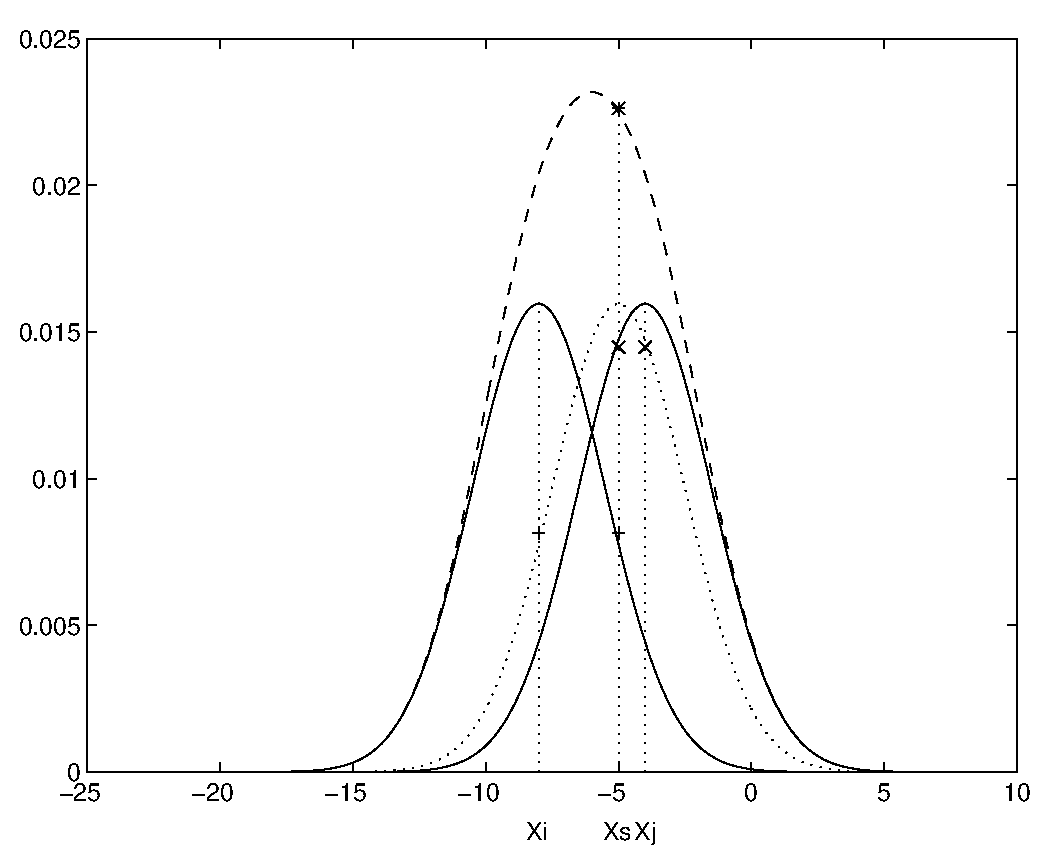
\includegraphics[height=6.2cm]{Assets/figure_ex.eps}
\caption{This is the caption of the figure}
\end{figure}

Since $u_{1}$ is a smooth function, we will have
$\left\|hu_{1}\right\|_\infty \le \eta$
for $h$ small enough, and inequality (\ref{eq:two}) will hold,
yielding thereby:
\begin{equation}
  \psi (hu_{1}) \le \frac{h^{2}}{2}
  \frac{1}{\lambda} \left\|u_{1} \right\|_{2}^{2} + \frac{h^{2}}{2}
  \frac{1}{\delta '} \left\|u_{1}\right\|^{2}\ .
\end{equation}

If we choose $\delta '$ close enough to $\delta$, the quantity
$\left(\frac{1}{\lambda} + \frac{1}{\delta '}\right)$
will be negative, and we end up with
\begin{equation}
  \psi (hu_{1}) < 0\ \ \ \ \ {\rm for}\ \ h\ne 0\ \ {\rm small}\ .
\end{equation}

On the other hand, we check directly that $\psi (0) = 0$. This shows
that 0 cannot be a minimizer of $\psi$, not even a local one.
So $\overline{u} \ne 0$ and
$\overline{u} \ne \Lambda_{o}^{-1} (0) = 0$. \qed
\end{proof}
%
\begin{corollary}
Assume $H$ is $C^{2}$ and
$\left(a_{\infty},b_{\infty}\right)$-subquadratic at infinity. Let
$\xi_{1},\allowbreak\dots,\allowbreak\xi_{N}$  be the
equilibria, that is, the solutions of $H' (\xi ) = 0$.
Denote by $\omega_{k}$
the smallest eigenvalue of $H'' \left(\xi_{k}\right)$, and set:
\begin{equation}
  \omega : = {\rm Min\,} \left\{\omega_{1},\dots,\omega_{k}\right\}\ .
\end{equation}
If:
\begin{equation}
  \frac{T}{2\pi} b_{\infty} <
  - E \left[- \frac{T}{2\pi}a_{\infty}\right] <
  \frac{T}{2\pi}\omega
  \label{eq:three}
\end{equation}
then minimization of $\psi$ yields a non-constant $T$-periodic solution
$\overline{x}$.
\end{corollary}
%

We recall once more that by the integer part $E [\alpha ]$ of
$\alpha \in \bbbr$, we mean the $a\in \bbbz$
such that $a< \alpha \le a+1$. For instance,
if we take $a_{\infty} = 0$, Corollary 2 tells
us that $\overline{x}$ exists and is
non-constant provided that:

\begin{equation}
  \frac{T}{2\pi} b_{\infty} < 1 < \frac{T}{2\pi}
\end{equation}
or
\begin{equation}
  T\in \left(\frac{2\pi}{\omega},\frac{2\pi}{b_{\infty}}\right)\ .
  \label{eq:four}
\end{equation}

%
\begin{proof}
The spectrum of $\Lambda$ is $\frac{2\pi}{T} \bbbz +a_{\infty}$. The
largest negative eigenvalue $\lambda$ is given by
$\frac{2\pi}{T}k_{o} +a_{\infty}$,
where
\begin{equation}
  \frac{2\pi}{T}k_{o} + a_{\infty} < 0
  \le \frac{2\pi}{T} (k_{o} +1) + a_{\infty}\ .
\end{equation}
Hence:
\begin{equation}
  k_{o} = E \left[- \frac{T}{2\pi} a_{\infty}\right] \ .
\end{equation}

The condition $\gamma < -\lambda < \delta$ now becomes:
\begin{equation}
  b_{\infty} - a_{\infty} <
  - \frac{2\pi}{T} k_{o} -a_{\infty} < \omega -a_{\infty}
\end{equation}
which is precisely condition (\ref{eq:three}).\qed
\end{proof}
%

\begin{lemma}
Assume that $H$ is $C^{2}$ on $\bbbr^{2n} \setminus \{ 0\}$ and
that $H'' (x)$ is non-de\-gen\-er\-ate for any $x\ne 0$. Then any local
minimizer $\widetilde{x}$ of $\psi$ has minimal period $T$.
\end{lemma}
%
\begin{proof}
We know that $\widetilde{x}$, or
$\widetilde{x} + \xi$ for some constant $\xi
\in \bbbr^{2n}$, is a $T$-periodic solution of the Hamiltonian system:
\begin{equation}
  \dot{x} = JH' (x)\ .
\end{equation}

There is no loss of generality in taking $\xi = 0$. So
$\psi (x) \ge \psi (\widetilde{x} )$
for all $\widetilde{x}$ in some neighbourhood of $x$ in
$W^{1,2} \left(\bbbr / T\bbbz ; \bbbr^{2n}\right)$.

But this index is precisely the index
$i_{T} (\widetilde{x} )$ of the $T$-periodic
solution $\widetilde{x}$ over the interval
$(0,T)$, as defined in Sect.~2.6. So
\begin{equation}
  i_{T} (\widetilde{x} ) = 0\ .
  \label{eq:five}
\end{equation}

Now if $\widetilde{x}$ has a lower period, $T/k$ say,
we would have, by Corollary 31:
\begin{equation}
  i_{T} (\widetilde{x} ) =
  i_{kT/k}(\widetilde{x} ) \ge
  ki_{T/k} (\widetilde{x} ) + k-1 \ge k-1 \ge 1\ .
\end{equation}

This would contradict (\ref{eq:five}), and thus cannot happen.\qed
\end{proof}
%
\paragraph{Notes and Comments.}
The results in this section are a
refined version of \cite{smit:wat};
the minimality result of Proposition
14 was the first of its kind.

To understand the nontriviality conditions, such as the one in formula
(\ref{eq:four}), one may think of a one-parameter family
$x_{T}$, $T\in \left(2\pi\omega^{-1}, 2\pi b_{\infty}^{-1}\right)$
of periodic solutions, $x_{T} (0) = x_{T} (T)$,
with $x_{T}$ going away to infinity when $T\to 2\pi \omega^{-1}$,
which is the period of the linearized system at 0.

\begin{table}
\caption{This is the example table taken out of {\it The
\TeX{}book,} p.\,246}
\begin{center}
\begin{tabular}{r@{\quad}rl}
\hline
\multicolumn{1}{l}{\rule{0pt}{12pt}
                   Year}&\multicolumn{2}{l}{World population}\\[2pt]
\hline\rule{0pt}{12pt}
8000 B.C.  &     5,000,000& \\
  50 A.D.  &   200,000,000& \\
1650 A.D.  &   500,000,000& \\
1945 A.D.  & 2,300,000,000& \\
1980 A.D.  & 4,400,000,000& \\[2pt]
\hline
\end{tabular}
\end{center}
\end{table}
%
\begin{theorem} [Ghoussoub-Preiss]\label{ghou:pre}
Assume $H(t,x)$ is
$(0,\varepsilon )$-subquadratic at
infinity for all $\varepsilon > 0$, and $T$-periodic in $t$
\begin{equation}
  H (t,\cdot )\ \ \ \ \ {\rm is\ convex}\ \ \forall t
\end{equation}
\begin{equation}
  H (\cdot ,x)\ \ \ \ \ {\rm is}\ \ T{\rm -periodic}\ \ \forall x
\end{equation}
\begin{equation}
  H (t,x)\ge n\left(\left\|x\right\|\right)\ \ \ \ \
  {\rm with}\ \ n (s)s^{-1}\to \infty\ \ {\rm as}\ \ s\to \infty
\end{equation}
\begin{equation}
  \forall \varepsilon > 0\ ,\ \ \ \exists c\ :\
  H(t,x) \le \frac{\varepsilon}{2}\left\|x\right\|^{2} + c\ .
\end{equation}

Assume also that $H$ is $C^{2}$, and $H'' (t,x)$ is positive definite
everywhere. Then there is a sequence $x_{k}$, $k\in \bbbn$, of
$kT$-periodic solutions of the system
\begin{equation}
  \dot{x} = JH' (t,x)
\end{equation}
such that, for every $k\in \bbbn$, there is some $p_{o}\in\bbbn$ with:
\begin{equation}
  p\ge p_{o}\Rightarrow x_{pk} \ne x_{k}\ .
\end{equation}
\qed
\end{theorem}
%
\begin{example} [{{\rm External forcing}}]
Consider the system:
\begin{equation}
  \dot{x} = JH' (x) + f(t)
\end{equation}
where the Hamiltonian $H$ is
$\left(0,b_{\infty}\right)$-subquadratic, and the
forcing term is a distribution on the circle:
\begin{equation}
  f = \frac{d}{dt} F + f_{o}\ \ \ \ \
  {\rm with}\ \ F\in L^{2} \left(\bbbr / T\bbbz; \bbbr^{2n}\right)\ ,
\end{equation}
where $f_{o} : = T^{-1}\int_{o}^{T} f (t) dt$. For instance,
\begin{equation}
  f (t) = \sum_{k\in \bbbn} \delta_{k} \xi\ ,
\end{equation}
where $\delta_{k}$ is the Dirac mass at $t= k$ and
$\xi \in \bbbr^{2n}$ is a
constant, fits the prescription. This means that the system
$\dot{x} = JH' (x)$ is being excited by a
series of identical shocks at interval $T$.
\end{example}
%
\begin{definition}
Let $A_{\infty} (t)$ and $B_{\infty} (t)$ be symmetric
operators in $\bbbr^{2n}$, depending continuously on
$t\in [0,T]$, such that
$A_{\infty} (t) \le B_{\infty} (t)$ for all $t$.

A Borelian function
$H: [0,T]\times \bbbr^{2n} \to \bbbr$
is called
$\left(A_{\infty} ,B_{\infty}\right)$-{\it subquadratic at infinity}
if there exists a function $N(t,x)$ such that:
\begin{equation}
  H (t,x) = \frac{1}{2} \left(A_{\infty} (t) x,x\right) + N(t,x)
\end{equation}
\begin{equation}
  \forall t\ ,\ \ \ N(t,x)\ \ \ \ \
  {\rm is\ convex\ with\  respect\  to}\ \ x
\end{equation}
\begin{equation}
  N(t,x) \ge n\left(\left\|x\right\|\right)\ \ \ \ \
  {\rm with}\ \ n(s)s^{-1}\to +\infty\ \ {\rm as}\ \ s\to +\infty
\end{equation}
\begin{equation}
  \exists c\in \bbbr\ :\ \ \ H (t,x) \le
  \frac{1}{2} \left(B_{\infty} (t) x,x\right) + c\ \ \ \forall x\ .
\end{equation}

If $A_{\infty} (t) = a_{\infty} I$ and
$B_{\infty} (t) = b_{\infty} I$, with
$a_{\infty} \le b_{\infty} \in \bbbr$,
we shall say that $H$ is
$\left(a_{\infty},b_{\infty}\right)$-subquadratic
at infinity. As an example, the function
$\left\|x\right\|^{\alpha}$, with
$1\le \alpha < 2$, is $(0,\varepsilon )$-subquadratic at infinity
for every $\varepsilon > 0$. Similarly, the Hamiltonian
\begin{equation}
H (t,x) = \frac{1}{2} k \left\|k\right\|^{2} +\left\|x\right\|^{\alpha}
\end{equation}
is $(k,k+\varepsilon )$-subquadratic for every $\varepsilon > 0$.
Note that, if $k<0$, it is not convex.
\end{definition}
%

\paragraph{Notes and Comments.}
The first results on subharmonics were
obtained by Rabinowitz in \cite{fo:kes:nic:tue}, who showed the existence of
infinitely many subharmonics both in the subquadratic and superquadratic
case, with suitable growth conditions on $H'$. Again the duality
approach enabled Clarke and Ekeland in \cite{may:ehr:stein} to treat the
same problem in the convex-subquadratic case, with growth conditions on
$H$ only.

Recently, Michalek and Tarantello (see \cite{fost:kes} and \cite{czaj:fitz})
have obtained lower bound on the number of subharmonics of period $kT$,
based on symmetry considerations and on pinching estimates, as in
Sect.~5.2 of this article.
% 1. Введение
Система AlgoView позволяет составить информационный граф алгоритма [1], на основе его описания на языке Algolang [2]. Система создает интерактивную 3D модель заданного алгоритма и предоставляет возможности по его анализу [3]. Такой функционал обеспечивает активное применение системы в образовательных и исследовательских целях [4].
Автоматизированная система визуализации призвана обеспечить визуальное представление внутренней структуры алгоритма, облегчить процесс детального анализа алгоритма и освободить от необходимости вручную выполнять визуализацию алгоритма, обеспечивая исследователям возможность сосредоточиться на анализе алгоритма. Для достижения этих целей интерактивная 3D модель графа алгоритма содержит вспомогательную информацию, обеспечивающую максимальную наглядность принадлежности дуг отдельным вершинам и общей логической структуры алгоритма. Это позволяет работать с системой визуализации и тем, кто не имеет опыта в области применения интересующего алгоритма.
В данной статье описана разработка новой версии системы AlgoView. Произведен обзор существующих решений для построения вычислительной части и способов интерактивной 3D визуализации с возможностями анализа.
2. Постановка задачи
2.1. План работы
Целью проекта является исследование современных методов и разработка новой версии системы AlgoView. Требуется провести исследования для реализации вычислительной составляющей системы. Так же требуется провести исследование современных методов 3D визуализации и разработать автоматизированную систему визуализации графов алгоритмов. Для достижения поставленных целей необходимо пройти многоэтапный процесс исследований и разработки и выполнить следующие задачи:
Изучить понятие информационного графа алгоритма, его свойства и способы применения и анализа, изучить способы описания графа алгоритма. Рассмотреть синтаксис языка Algolang, предназначенного для описания информационной структуры алгоритма в виде XML-файла. По возможности сделать язык Algolang более универсальным.
Изучить возможные методы обработки и программные библиотеки для работы с информационными структурами формата XML, а так же способы вычисления математических выражений, задаваемых в текстовом виде, используемых при описании информационных графов алгоритмов.
Разработать программные методы для обработки необходимой информации об алгоритме из описания на языке Algolang.
Разработать новый формат хранения данных об алгоритме, на основе которого информационный граф может быть визуализирован без дополнительных вычислений с целью получения необходимой информации о структуре графа.
Реализовать программный алгоритм, который на основе информации, полученной из описания алгоритма на языке Algolang, составляет описание модели многомерного графа по новому формату, по которой он может быть визуализирован. Модель должна представлять собой описание расположения вершин и дуг графа в пространстве, а также характеристики информационного графа и свойства каждого элемента этого графа.
Сформировать архитектуру приложения и понятия внутреннего представления графа алгоритма в системе визуализации AlgoView.
Создание программного средства, преобразующего промежуточное представление графа алгоритма формата JSON в множество 3D моделей.
Реализация программного обеспечения, производящего интерактивную 3D визуализацию множества сформированных объектов, представляющих собой граф алгоритма.
Создание web-страницы, на которой производится визуализация и взаимодействие с интерфейсом.
2.2. Промежуточный формат данных
Система Algoview разделяется на вычислительную часть и задачу визуализации. Для автоматизации работы системы требуется разработка нового формата хранения данных об алгоритме. В качестве стандартизированного представления графа алгоритма выступает JSON структура, содержащая характеристики информационного графа алгоритма, информацию о координатах и типе вершин, и информацию о связанности этих вершин через их уникальные идентификаторы. Разработанная структура данных имеет следующий вид (пример из трех вершин и 2 дуг):

Fig. 1: JSON структура, пример исходного формата данных и пример визуализации этого графа.
2.3. [Глеб] Стандарт визуализации графов алгоритмов
Стандарт визуализации графов алгоритмов — стандарт, впервые описанный как руководство, состоящее из набора правил, в соответствии с которыми рекомендуется изображать граф алгоритма. Существование стандарта обуславливается потребностью в построении изображений графов алгоритмов в общепринятом виде, который будет понятен вне зависимости от инструментов, используемых для изображения графа [5]. С появлением системы AlgoView, как универсального способа генерации изображений графов алгоритмов, многие положения в стандарте требуют пересмотра. Нововведения в стандарте касаются автоматизации процесса и ослабления строгости требований к изображению графов.
3. Исследование методов и построение решения
3.1. [Тамара] Обзор существующих решений обработки файлов формата XML
Синтаксические анализаторы SAX и DOM.
Существует два основных подхода анализа файлов формата XML - DOM и SAX API (Application Programming Interface).
DOM анализаторы осуществляют обработку XML-файла, предварительно загрузив данные этого файла в программу в виде DOM (Document Object Model) дерева [6]. Оно является представлением HTML-документа в виде дерева тегов.
SAX (Simple API for XML) анализаторы, в свою очередь, осуществляют поточную событийную обработку XML-документов, не загружая данные во внутренние структуры программы [7].
В качестве целевого варианта рассматривались библиотеки, предлагающие DOM API, поскольку в рамках данной работы потоков обработка не требуется.
Библиотеки, предоставляющие DOM API для обработки XML-файлов.
Наиболее используемыми для языка C++ библиотеками, предоставляющими DOM API, являются RapidXML, PugiXML, TinyXML [9].
RapidXML в основном ориентирован на уменьшение времени выполнения и представляет собой стабильный и быстрый парсер, работающий со скоростью приближающейся к скорости работы функции strlen (функция подсчёта длины в байтах), выполняемой на тех же данных [10].
PugiXML — это библиотека, которая предоставляет программный интерфейс DOM с широкими возможностями обхода/модификации, чрезвычайно быстрый синтаксического анализатор, и возможность доступа к данным по заданному пути [11].
TinyXML — это минимальная версия для анализа данных XML-файлов, не такая быстрая, как две предыдущие. Данная библиотека была создана из соображений простоты в использовании и освоении, и хорошо подходит в том случае, если большая скорость выполнения не является приоритетным фактором при выборе инструментов для работы [12].
Компилятор привязки данных.
Помимо SAX и DOM анализаторов существует способ обработки при помощи компилятора привязки данных XSD Schema. Такой способ был предложен компанией CodeSynthesis, как альтернативное решение обработки XML-файлов с некоторыми преимуществами по сравнению с традиционными подходами [14]. При наличии спецификации экземпляра XML (XML-схема) он генерирует классы C++, представляющие заданный словарь, а также код синтаксического анализа и сериализации XML. По сравнению с API-интерфейсами, такими как DOM и SAX, привязка данных XML позволяет пользователю получать доступ к данным в XML-документах, используя сгенерированный доменный словарь, а не общие элементы, атрибуты и текст.
Дополнительные решения для обработки XML-файлов.
Помимо способов работы напрямую с XML-файлами существует возможность осуществления тех же действий (доступ/анализ/обработка) с данными, только предварительно осуществив конвертацию XML формата к JSON (JavaScript Object Notation) — стандартному текстовому формату обмена данными. В таком случае для обработки данных уже используются библиотеки для работы с форматом JSON, самой используемой из них является RapidJSON.
Важным в рамках данной работы оказался способ представления данных при работе с программным интерфейсом DOM. RapidJSON работает с сущностью Value, которая может быть двух типов — Object и Array. С точки зрения исходного XML-файла — все его теги являются объектами и все одноимённые теги объединяются в массивы. Таким образом, древовидная структура, в виде которой данные хранятся в программе, у библиотеки RapidJSON отличается от структур библиотек, работающих напрямую с форматом XML [15]. И тогда обход этой древовидной структуры, а в частности переход между разноимёнными тегами, расположенными на одной глубине, отличается и представляется более удобным и безопасным с точки зрения доступа к памяти.
3.2. [Тамара] Обзор библиотек для вычисления значений математических выражений
В рамках работы системы визуализации существует необходимость вычисления и оценки математических выражений, с помощью которых описывается информационная структура алгоритма. Для этих целей на языке C++ существует набор внедряемых в проекты сторонних библиотек с открытым кодом. Самыми используемыми и подходящими в рамках данной работы являются ExprTk, muParser, METL (Math Expression Toolkit Library).
Библиотека ExprTk.
ExprTk является наиболее полной и используемой библиотекой для разбора и оценки математических выражений из приведённых выше. Механизм синтаксического анализа поддерживает множество форм функциональной и логической семантики обработки и легко расширяется. Библиотека ExprTk позволяет работать со скалярными, строковыми и векторными типами  данных с числовыми типами Float, Double и MPFR (multiple-precision floating-point) и поддерживает обработку различных математических операций и функций [17]. ExprTk работает по принципу разбора выражения в AST дерево, что позволяет оценить его значение. Согласно тестам производительности, библиотека считается самым быстрым решением для вычисления стандартных операций со скалярными значениями.
Серия библиотек muParser.
MuParser — это серия расширяемых высокопроизводительных библиотек, предоставляющих пользователю разные возможности в зависимости от его нужд [19]. Для достижения большей скорости работы со скалярными значениями с ограничением на количество и тип используемых параметров и точность вычислений используется библиотека muparserSSE. Для преодоления данных ограничений с увеличением времени работы используется muparser. Для работы с векторными и строковыми типами данных и комплексными числами применима версия библиотеки muparserX.
Библиотека METL.
Math Expression Toolkit Library — небольшая библиотека для стандарта языка c++14 для анализа математических выражений. Она спроектирована таким образом, чтобы быть достаточно гибкой, но и то же время эффективной. Под гибкостью подразумевается, что выражения могут использовать все типы переменных с разумным поведением (например, полезно для работы с векторами и матрицами) и при этом добавление и редактирование операторов и функций очень просто.
Сравнение библиотек.
Для библиотек осуществлено сравнение с помощью тестов производительности, разработанных для тестирования корректности вычислений и скорости работы библиотек для парсинга математических выражений, написанных на языке C++ и работающих по принципу POEM (Parse Once Evaluate Many times) [22]. По результатам замеров времени вычислений лидерами среди библиотек для парсинга математических выражений являются muparserSSE и ExprTkFloat, работающие с типом данных Float, а с учётом также точности вычислений - ExprTk, работающая с типом данных  Double [22].
3.3. [Глеб] Исследование методов 3D визуализации
Трехмерная визуализация — важный аспект взаимодействия с пользователем при разработке программного обеспечения. В настоящее время проводится много исследований в области визуализаций графов [23][24][25][26]. Однако анализ производительности алгоритмов с использованием информационных графов не является достаточно популярной областью в науке и не содержит устоявшиеся методов. Для понимания способов реализации проекта требуется дополнительное рассмотрение популярных технологий трехмерной визуализации, доступных на сегодняшний день. В ходе исследования доступных методов 3D-визуализации, были рассмотрены около 10 различных решений: OpenGL [28], WebGL [29][30][31], Three.js [32][33], Babylon.js [34], VTK (Visualization Toolkit) [35], OpenSceneGraph [36], DirectX [37], Unity [38], Blender [39], Maya [40].
После сравнительного анализа инструментов визуализации был сделан вывод, что самые простые и удобные методы визуализации графов реализованы во фреймворках Three.js, Babylon.js, а также на платформе Unity. Итоговый выбор был сделан в пользу фреймворка Three.js, за счет своей легковесности и кроссбраузерности. Для контроля над сценой был использован модуль OrbitControls. Данный модуль является самым распространенным и поддерживаемым решением для реализации управления при помощи компьютерной мышки и клавиатуры [43]. Для создания пользовательского интерфейса и меню управления с возможностями дополнительного анализа графов алгоритмов был использован легковесный модуль dat.GUI [44]. Размер библиотеки со всеми дополнительными модулями пользовательского интерфейса не превышает 1 мегабайта.
3.4. [Глеб] Метод изгиба дуг в трехмерном пространстве
Показатель необходимости изгиба дуг.
Главным сигналом необходимости изгиба дуги возникает при пересечении вершины прямой дугой, так как в этом случае часто непонятно, откуда и куда выходит дуга. Пересечение разных дуг или прохождение дуги через оболочку 3D объекта вершины в среднем не создают проблем с визуальным восприятием информационного графа.
Математический смысл изгиба дуги.
Пусть в трехмерной декартовой системе координат $\Phi$ с базисными векторами $\overrightarrow{i}, \overrightarrow{j}, \overrightarrow{k}$имеется 2 вершины: $A(x_1; y_1; z_1)$ и $B(x_2; y_2; z_2)$. Обозначим длину вектора $\overrightarrow{AB}$ как $len = \sqrt{ (x_2 - x_1)^2 + (y_2 - y_1)^2 + (z_2 - z_1)^2 }$. Пусть между вершинам $A$ и $B$ есть отрезок, которую требуется геометрически изогнуть. Изгибая дугу между вершинами можем представить что вектор $\overrightarrow{AB}$ является одним из базисных векторов другой трехмерной декартовой системы координат $\Psi$, в который нам требуется описать уравнение кривой, исходящей из точки $A(0; 0; 0)$, то есть начала координат, и приходящей в точку $B\left(len; 0; 0 \right)$, удаленную от начала координат на расстояние $len$. После описания уравнения кривой можно перейти к изначальному базису, позиционирующему кривую в пространстве так, чтобы она соответствовала вершинам $A$ и $B$ в изначальной системе координат $\Phi$.
Геометрический метод нахождения базиса.
Вектор $\overrightarrow{AB}$ в трехмерной системе координат $\Phi$ соответствует отрезку $AB$ и является одним из базисных векторов в системе координат $\Psi$. Вычислим первый единичный базисный вектор $\overrightarrow{n_1}$:
$$ \overrightarrow{n_1} = \frac {\overrightarrow{AB}} {\left|\overrightarrow{AB}\right|} $$
Для нахождения второго единичного базисного вектора $\overrightarrow{n_2}$ воспользуемся геометрическими и тригонометрическими методами:
$$ b = \frac {\left|y_{n_1}\right|} {\tg( \frac{\pi}{2} -\sin(\left|x_{n_1}\right|) )}; \quad \gamma = \arctg\left( \left| \frac{z_{n_1}}{x_{n_1}} \right| \right); $$
$$ \overrightarrow{n_2} = \left\{ -b\cos(\gamma) \frac{x_{n_1}} {\left|x_{n_1}\right|}; \quad y_{n_1}; \quad -b\sin(\gamma) \frac{z_{n_1}} {\left|z_{n_1}\right|} \right\} $$
Для нахождения третьего единичного базисного вектора $\overrightarrow{n_3}$ используем векторное произведение:
$$ \overrightarrow{n_3} = \overrightarrow{n_1} \times \overrightarrow{n_2} $$
Единичные вектора $\{\overrightarrow{n_1}, \overrightarrow{n_2}, \overrightarrow{n_3}\}$ образуют базис трехмерной декартовой системы координат $\Psi$.
Метод изгиба дуг через параметрически заданную окружность.
Изгиб дуги при помощи нахождения параметрического уравнения кривой происходит в вышеописанной трехмерной декартовой системе координат $\Psi$. Оптимальным видом изогнутой дуги является часть окружности, ограниченная точками $A(0; 0; 0)$, $B\left(len; 0; 0 \right)$. Для получения искомой дуги достаточно воспользоваться стандартным методом нахождения уравнения окружности по заданному центру и радиусу.
$$ x = R\cos\theta + x_{center}; \quad y = R\sin\theta + y_{center} $$
Радиус описываемой окружности $R$ имеет линейную зависимость от величины расстояния $len$. Центр окружности $C(x_{center}; y_{center}; 0)$ и диапазон значений параметра $\theta$ вычисляются геометрически.
4. Построение архитектуры и алгоритм работы системы AlgoView, программная реализация
4.1. Схема работы системы AlgoView
Работа приложения состоит из множества шагов, которые протекают автоматически. Рассмотрим последовательность действий системы, начиная с загрузки в систему файла с описанием информационной структуры алгоритма на языке Algolang, до получения интерактивной 3D модели информационного графа данного алгоритма.
Работа вычислительной подпрограммы.
В качестве входных данных система принимает описание алгоритмов на языке Algolang в формате XML. ****Далее происходит конвертация исходного файла в формат JSON. Следующим этапом, при помощи средств библиотеки RapidJSON, в памяти создаётся древовидная структура DOM, по которой возможен доступ ко всем данных первоначального XML файла. По данной структуре производится обход с целью сбора всей информации о графе в программные классы с выполнением некоторых промежуточных вычислений для удобства использования, а именно осуществление вычисления диапазонов значений пространства итераций. Для подсчёта значений данных выражений используется библиотека ExprTk. Вычисление всех имеющихся в описании алгоритма выражений на данном этапе невозможно, поскольку они обладают зависимостью от текущих значений пространства итераций и будут вычисляться в дальнейшем. Такие выражения при обходе сохраняются в виде строк без изменений в качестве атрибутов экземпляра класса. После сбора всех данных входного файла и проведения предварительной обработки, запускается основной цикл, выполняющий содержательную работу всей программы. Внутри него происходит проход по всему пространству итераций, осуществляются вычисления, зависимые от текущих его значений, происходит формирование координат вершин, определение их уровня ярусно-параллельной формы [41] и определение вершин, связанных информационной дугой.
По результатам работы этого этапа формируются списки экземпляров классов вершин и дуг с описанием их свойств, общая информация о графе и/или списки предупреждений и ошибок (при наличии). Далее, на основе этой информации, формируется файл с JSON структурой в качестве формата промежуточных данных, который используется в дальнейшем для построения интерактивной 3D визуализации.
Работа подпрограммы визуализации.
После создания промежуточного файла, пользователь получает веб-страницу с приложением визуализации, которое запускается автоматически после загрузки. Первым шагом программа преобразовывает данные из JSON структуры с промежуточными данными и составляет из них внутреннюю структуру графа. Далее производится создание 3D представления графа в виде множества 3D объектов, соответствующих и визуально описывающих все структурные элементы графа. Последним этапом является построение интерактивной визуализации полученного набора 3D-моделей, образуя вместе с пользовательских интерфейсом многофункциональную систему анализа.
4.2 Этапы работы вычислительной подпрограммы
Для начала сделаем несколько оговорок. В процессе описания работы вычислительной части системы визуализации используемое понятие ярусно-параллельной формы информационного графа будет подразумевать именно каноническую ЯПФ этого графа. Информационный граф алгоритма, построенный в результате работы программы не является таковым в классическом его понимании, поскольку содержит в себе также и вершины с входными данными, что противоречит определению, в котором вершинами являются только операции алгоритма. То есть понятие графа, используемое в рамках реализованной программы, является как бы надграфом, образованным путём добавления к графу алгоритма вершин с входными данными. Также существует ограничение, накладываемое на входные данные, а именно для блоков алгоритма(тег <block> на языке Algolang), описывающих опорные многогранники его графа, наложено ограничение не более чем трёхмерной размерности.
Конвертация в JSON.
На первом этапе работы происходит мгновенная конвертация XML-файла в JSON с помощью небольшой библиотеки xml2json. Таким образом, ошибкой, обрабатывающей этим этапом, может быть только неверная структура XML-файла.
Сбор входных данных.
На этапе сбора входных данных для обхода входного файла применяется предоставленный библиотекой RapidJSON API DOM. Библиотека выбрана в связи с более безопасным способом доступа к вершинам DOM дерева, построенного на основе XML, который исключил возникавшие с языком Algolang проблемы перехода по пустому указателю. В результате обхода DOM дерева создаются программные классы, содержащие всю нужную информацию об информационной структуре алгоритма. Также библиотека имеет встроенные средства для обработки ошибок, с помощью которых была реализована валидация входных данных (например, повторное использование имени аргумента внутри одного блока, заданы некорректные границы аргументов и т.д.).
Вычисление математических и условных выражений.
Возможность вычисления математических и условных выражений необходимо для обработки выражений, описанных во входных данных. Инструментом для этих целей была выбрана библиотека ExprTk, которая легко интегрируется в проекты и предлагает большую базу обрабатываемых функций и операций, а также быстро выполняет вычисления. Все вычисления в программе осуществляются одной отдельной функцией, принимающей на вход выражение в виде строки и карту имён и значений параметров, участвующих в вычислении.
Основной цикл.
Так называемый “Основной цикл” программы осуществляет содержательную её часть и формирует программные классы с итоговой информацией о модели графа алгоритма, которые достаточно переписать в некотором стандартном виде для возможности дальнейшей визуализации.
Работа "Основного цикла" реализует обработку одного блока алгоритма, соответственно данный фрагмент программы также работает в цикле для всех блоков. Когда на обработку подаётся блок, как программный класс со всей информацией о нём, для создаётся поле id-номеров вершин будущего информационного графа на основе диапазонов пространства итераций и определяется сдвиг всех координат по одной оси в зависимости от размерности предыдущего блока, чтобы блоки не накладывались друг на друга. На каждом шаге итерации выбирается текущее значение координат. Далее в цикле проверяются условия существования вершин с помощью функции вычисления математических выражений для этих координат. Если условие выполняется, то для данных значений создаётся вершина, которой присваивается очередной порядковый id и, на основе информации, полученной из описания на языке Algolang, её тип, или, если тип не был указан, то ему присваивается значение по умолчанию. После этого осуществляется обработка всех вершин-источников, из которых дуга ведёт в текущую. Проверяется, существует ли эта вершина, путём поиска её в поле id-номеров вершин блока, к которому она принадлежит, по заданным координатам. Если такой вершины не существует, значит она не является операцией алгоритма, а обозначает зависимость от входных данных. Такая вершина создаётся со специально определённым типом входных данных (тип "0") и значению уровня ярусно-параллельной формы данной вершины присваивается нуль. Если такая вершина существовала, то по её координатам программа получается id, также обращаясь к полю вершин. После этого для каждой вершины-источника, по её id и id текущей вершины, создаётся дуга. После обработки всех вершин-источников, для текущей вершины возможно определение уровня её ярусно параллельной формы. Далее происходит следующая итерация цикла.
Формирование промежуточных выходных данных.
В результате работы “основного цикла” программа формирует список объектов программных классов вершин и дуг с описанием их свойств. На основе этих списков формируются выходные данные в формате JSON. Таким образом, выходные данные реализованной программы представляют собой список вершин и дуг с перечислением их свойств, перечисление свойств графа и перечисление ошибок и/или предупреждений (при наличии). Для Вершин — это id, координаты, тип и уровень ярусно-параллельной формы, для дуг — id, id вершин, которые она соединяет, с направлением от первой названной вершины ко второй, и тип, для графа — количество вершин и дуг, длина критического пути и ширина ярусно-параллельной формы.
Расчет ярусно параллельной формы.
Одной из важнейших возможностей системы является отображения принадлежности групп вершин к уровням ярусно-параллельной форме. Это позволяет анализировать, какие операции алгоритма могут выполняться независимо друг от друга (параллельно, за один так времени). Определение уровня ЯПФ для каждой вершины происходит, как уже упоминалось ранее, в рамках работы “Основного цикла” по следующему принципу:
При создании новой вершины значением по умолчанию является уровень 0 ярусно-параллельной формы, что означает, что она не принадлежит никакому ярусу, то есть не является операцией (таким типом вершин является вершина входных данных)


Определятся, является ли данная вершина операцией или входными данными, и во втором случае ей присваивается уровень 1 ярусно-параллельной формы


Происходит сбор данных об уровне ярусно-параллельной формы всех вершин-источников, если таковые имеются, и вычисляется уровень текущей вершины по формуле

 $$ level = \max\left\{level(v): v \in source\_vertices\right\} + 1 $$


Анализ графа для формирования списка ошибок и предупреждений.
Система способна осуществлять анализ и обработку трёх видов ошибок. Системные критические ошибки оповещают пользователя о том, что произошла системная ошибка и повлиять на результат работы программы он не может. Такой тип ошибок возникает редко и создан для разработчика. Пользовательские критические ошибки оповещают пользователя по какой причине входные данные не могут быть обработаны. Пользователь может изменить содержание входного файлы для исключения ошибки. Некритические ошибки в результате работы системы визуализации возвращают граф построенный в соответствии с XML описанием графа, но с возможным наличием в нём ошибок, о которых пользователь получает предупреждение.
Принцип расположения вершин и дуг в пространстве.
Для расположения вершин и дуг информационного графа алгоритма в трёхмерном пространстве был выбран следующий принцип. Вводится трёхмерная декартова система координат и сетка фиксированного размера на ней, зависящая от диапазона значений пространства итераций. Далее, любая вершина графа алгоритма располагается в уникальном узле сетки и задаётся координатами этого узла. Любая дуга задаётся парой узлов сетки - её началом и концом. Таким способом можно отобразить в трёхмерной пространстве любой информационный граф алгоритма без наложений вершин. Для определения принадлежности вершины к уровню ярусно-параллельной формы используются средства интерактивной визуализации итоговой модели.
4.3. [Глеб] Архитектура ПО для задачи визуализации
Одной из главных задач при программной реализации системы является выбор и разработка подходящей архитектуры приложения. От выбранной архитектуры зависит способ обработки данных и общения с пользователем. Выбор неподходящей структуры и методов общения модулей приложения между собой может значительно повысить нагрузку на ядро браузера и вычислительные ресурсы операционной системы. Рассмотрим основные модули системы визуализации для решения этой проблемы:
Работа с данными, считывание и создание внутренней структуры графа.
Работа со структурой графа, основываясь параметрах вида, задаваемых пользователем. Создание 3D моделей для каждого объекта в структуре графа.
Создание 3D сцены, содержащей модель графа.
Работа с пользователем: обеспечение связи панели управления с моделью графа, сценой и параметрам и вида.
При изменении параметров вида данные в модели должны локально изменяться и последовательно обновлять структуру графа и 3D модели, представляющие этот граф на сцене.
Описанные требования и основные функциональные части являются достаточными критериями для выбора архитектуры Model-View-Controller (MVC) [45].
Описание используемой архитектуры MVC.
Архитектура MVC представляет собой шаблон для реализации программного обеспечения, который разделяет работу с данными приложения, пользовательский интерфейс и логику управления на три взаимосвязанных самостоятельных компонента. Модель (Model) представляет данные и бизнес-логику приложения, Представление (View) представляет уровень представления приложения, а Контроллер (Controller) действует как посредник между Моделью и Представлением, обрабатывая пользовательский ввод и обновляя Модель и Представление по мере необходимости. Когда пользователь взаимодействует с приложением, контроллер получает входные данные и решает, как соответствующим образом обновить модель и представление. Модель отвечает за обработку данных и самообновление, а представление отображает данные пользователю в презентабельном формате. Эта архитектура помогает разбивать сложные приложения на более мелкие, более управляемые компоненты, упрощая разработку, тестирование и обслуживание приложения [46].
Разделение ответственности между модулями системы визуализации AlgoView.
В рассматриваемой системе визуализации AlgoView, используемая архитектура MVC состоит из модели (Model) со структурой графа, части отображения (View) с набором методов преобразования данных в 3D модели и контроллера (Controller), содержащего в себе методы изменения модели и обновления визуализации через пользовательский интерфейс. Выбрав архитектуру, требуется грамотно распределить задачи и ответственность между модулями приложения, следуя правилам конкретной архитектуры. Рассмотрим, как в данном случае распределена ответственность:
Содержание модуля Model: обработка входных данных; хранение внутренней структуры графа; обновление данных в структуре графа по командам пользователя.
Содержание модуля View: обеспечение набором методов преобразования данных в 3D модели; заполнение сцены 3D моделями, полученными из объектов графа, хранящимися в Model.
Содержание модуля Controller: создание графического пользовательского интерфейса; обеспечение связи между пользователем, его командами через меню управления и связкой Model-View; управление Model и View через их встроенные методы контроля.
5. Пример работы системы AlgoView
Разберем пример работы системы на простом алгоритме “Нахождение суммы элементов массива сдваиванием”. ****Метод сдваивания используется в качестве быстрого варианта вычисления длинных последовательностей ассоциативных операций. Элементы на каждом этапе алгоритма разбиваются на пары. В каждой из пар находится сумма составляющих её элементов. На следующем этапе на пары разбиваются уже эти суммы, и т. д. Характеристики алгоритма (для суммирования массива порядка n): общее количество вершин: $n - 1$ ; длина критического пути: $\left\lceil{\log_2n}\right\rceil$; каноническая ширина ЯПФ: $n$.
Последовательная сложность алгоритма. Для вычисления суммы массива, состоящего из $n$ элементов, при любых разложениях $n$ на пары суть алгоритма сводится к простому переставлению скобок в формуле суммирования. Количество операций неизменно и равно $n-1$. Последовательный алгоритм должен быть отнесён к алгоритмам линейной сложности по количеству последовательных операций.
Ресурс параллелизма алгоритма. Для суммирования массива порядка $n$ методом сдваивания в параллельном варианте требуется последовательно выполнить $\left\lceil{\log_2n}\right\rceil$ ярусов с убывающим (от $n/2$ до 1) количеством операций суммирования. При классификации по высоте ЯПФ, таким образом, метод сдваивания относится к алгоритмам с логарифмической сложностью. При классификации по ширине ЯПФ его сложность будет линейной.

Fig. 2: Работа системы AlgoView на примере алгоритма “Нахождение суммы элементов массива сдваиванием” для $n = 8$ от реализации алгоритма на языке Си до итоговой визуализации.
6. Заключение
В статье рассматривается исследование современных методов для разработки новой версии системы трехмерной визуализации и интерактивного анализа информационных графов алгоритмов AlgoView. Система в описанном виде используется для академических занятий студентами магистратуры, демонстрируем работоспособность и полезность для науки и исследования информационных графов алгоритмов. В статье показан полный процесс реализации системы и описание алгоритмов для ее работы. Проведено тестирование системы визуализации на большом количестве примеров для выявления проблем и их исправления. Архитектура системы построена с учетом будущих разработок и дополнительных модификаций. Работа над проектом продолжается в сторону расширения класса алгоритмов, которые система может обработать, и новых способов интерактивного анализа графов.




\section{Introduction}

The AlgoView system allows you to create an information graph of the algorithm \cite{m1}, based on its description in the Algolang language \cite{m2}. The system creates an interactive 3D model of a given algorithm and provides opportunities for its analysis \cite{m3}. This functionality ensures active use of the system for educational and research purposes, for example, within the AlgoWiki project \cite{m4,a1}.

The automated visualization system aims to provide a visual representation of the internal structure of the algorithm, facilitate the process of detailed algorithm analysis, and eliminate the need to manually visualize the algorithm, allowing researchers to focus on analyzing the algorithm. To achieve these goals, the interactive 3D model of the algorithm graph contains auxiliary information that provides maximum visibility of the edges belonging to individual vertices and the overall logical structure of the algorithm. This allows those who do not have experience in the application of the algorithm of interest to work with the visualization system.

This paper describes the development of a new version of the AlgoView system. A review of existing solutions for building the computational part and methods of interactive 3D visualization with analysis capabilities was carried out.
 % Введение
\section{Statement of the problem}

\subsection{Work plan}

The goal of the project is to study modern methods and develop a new version of the AlgoView system. Research is required to implement the computational part of the system. It is also required to conduct research on modern 3D visualization methods and develop an automated system for visualizing algorithm graphs. To achieve these goals, it is necessary to go through a multi-stage research and development process and complete the following tasks:

\begin{enumerate}
    \item Study the concept of an information graph of an algorithm, its properties and methods of application and analysis, study ways of describing the algorithm graph. Consider the syntax of the Algolang language, designed to describe the information structure of the algorithm in the form of an XML file. If possible, make the Algolang language more universal.
    \item Study possible processing methods and software libraries for working with information structures of the XML format, as well as methods for calculating mathematical expressions specified in text form, used in describing information graphs of algorithms.
    \item Develop software methods for processing the necessary information about the algorithm from the description in the Algolang language.
    \item Develop a new format for storing data about the algorithm, on the basis of which the information graph can be visualized without additional calculations in order to obtain the necessary information about the structure of the graph.
    \item Implement a software algorithm that, based on information obtained from the description of the algorithm in the Algolang language, composes a description of the multidimensional graph model in a new format, according to which it can be visualized. The model should be a description of the location of the vertices and edges of the graph in space, as well as the characteristics of the information graph and the properties of each element of this graph.
    \item Form the architecture of the application and the concepts of the internal representation of the algorithm graph in the AlgoView visualization system.
    \item Creation of a software tool that converts an intermediate representation of the algorithm graph in JSON format into a variety of 3D models.
    \item Implementation of software that produces interactive 3D visualization of a set of generated objects representing an algorithm graph.
    \item Creation of a web page on which visualization and interaction with the interface is carried out.
\end{enumerate}

\subsection{Intermediate data format}

The AlgoView system is divided into a computational and visualization parts. To automate the operation of the system, it is necessary to develop a new format for storing data about the algorithm. The standardized representation of the algorithm graph is a JSON structure containing the characteristics of the algorithm information graph, information about the coordinates and type of vertices, and information about the connectivity of these vertices through their unique identifiers. The developed data structure has the following form (fig.~\ref{fig1} shows an example of three vertices and 2 edges).

\begin{figure}
% \vspace{-0.5cm}
\centering
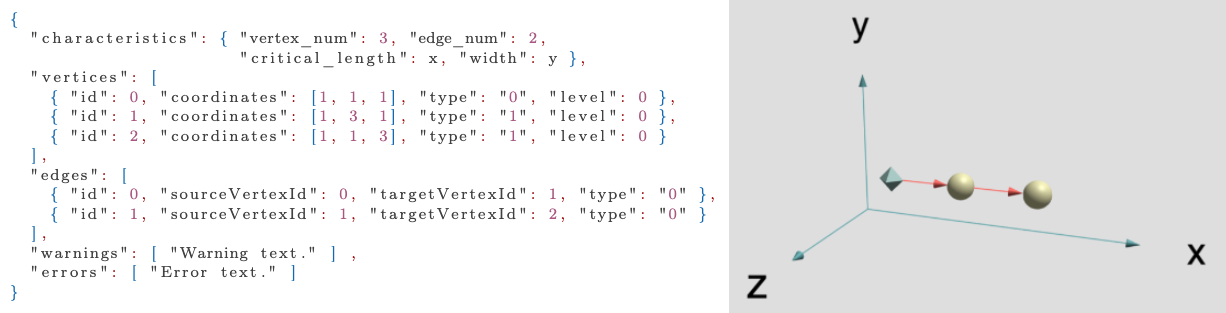
\includegraphics[height=3.1cm]{assets/json_example.png}
\caption{JSON structure, an example of the original data format and an example of visualization of this graph.}
\label{fig1}
\end{figure}

\subsection{Standard for visualizing algorithm graphs}

The Algorithm Graph Visualization Standard is a standard first described in the AlgoWiki project as a guide consisting of a set of rules according to which it is recommended to display an algorithm graph. The existence of the standard is determined by the need to construct images of algorithm graphs in a generally accepted form, which will be understandable regardless of the tools used to depict the graph. With the advent of the AlgoView system as a universal way to generate images of algorithm graphs, many provisions in the standard require revision. Innovations in the standard concern automation of the process and relaxation of the strict requirements for the image of graphs.
 % Постановка задачи
\section{Research methods and build a solution}

\subsection{Overview of existing solutions for processing XML files}

\textbf{SAX and DOM parsers.}

There are two main approaches to parsing XML files --- DOM and SAX APIs (Application Programming Interface).

DOM analyzers process an XML file by first loading the data of this file into the program in the form of a DOM (Document Object Model) tree \cite{m6}. It is a representation of an HTML document as a tree of tags.

SAX (Simple API for XML) analyzers, in turn, carry out stream-based event processing of XML documents without loading data into the internal structures of the program \cite{m7}.

Libraries that offer a DOM APIs were considered as a target option, since thread processing is not required for this work.

\textbf{Libraries that provide DOM APIs for processing XML files.} The most used libraries for the C++ language that provide the DOM API are RapidXML, PugiXML, TinyXML \cite{m9}.

RapidXML is primarily focused on reducing execution time and is a stable and fast parser that runs at speeds approaching the speed of the \texttt{strlen} function (a function that calculates the length in bytes) running on the same data \cite{m10}.

PugiXML is a library that provides a highly traversable/modifiable DOM programming interface, an extremely fast parser, and the ability to access data along a given path \cite{m11}.

TinyXML is a minimal version for parsing XML file data and is not as fast as the previous two. This library was created for reasons of ease of use and learning, and is well suited if high execution speed is not a priority factor when choosing tools for work \cite{m12}.

\textbf{Data binding compiler.} In addition to SAX and DOM analyzers, there is a way to process it using the XSD Schema data binding compiler. This method was proposed by Code Synthesis as an alternative solution for processing XML files with some advantages over traditional approaches \cite{m14}. Given an XML instance specification (XML Schema), it generates C++ classes representing the given vocabulary, as well as XML parsing and serialization code. Compared to APIs such as DOM and SAX, XML data binding allows the user to access data in XML documents using a generated domain vocabulary rather than generic elements, attributes, and text.

\textbf{Additional solutions for processing XML files.} In addition to the methods of working directly with XML files, it is possible to perform the same actions (access/analysis/processing) with data, only by first converting the XML format to JSON (JavaScript Object Notation) --- a standard text format for data exchange. In this case, libraries for working with the JSON format are already used to process the data, the most used of which is RapidJSON.

The method of presenting data when working with the DOM programming interface turned out to be important within the framework of this work. RapidJSON works with the Value entity, which can be of two types --- Object and Array. From the point of view of the source XML file, all its tags are objects and all tags of the same name are combined into arrays. Thus, the tree structure in which data is stored in the program in the RapidJSON library differs from the structures of libraries that work directly with the XML format \cite{m15}. And then bypassing this tree structure, and in particular the transition between tags of different names located at the same depth, is different and seems more convenient and safer from the point of view of memory access.

\subsection{Overview of libraries for calculating the values of mathematical expressions}

As part of the operation of the visualization system, there is a need to calculate and evaluate mathematical expressions that describe the information structure of the algorithm. For these purposes, in the C++ language, there is a set of third-party open source libraries implemented into projects. The most used and suitable for this work are ExprTk, muParser, METL (Math Expression Toolkit Library).

\textbf{ExprTk library.} ExprTk is the most complete and used library for parsing and evaluating the mathematical expressions above. The parsing engine supports many forms of functional and logical processing semantics and is easily extensible. The ExprTk library allows you to work with scalar, string and vector data types with numeric types Float, Double and MPFR (multiple-precision floating-point) and supports processing various mathematical operations and functions \cite{m17}. ExprTk works on the principle of parsing an expression in an AST tree, which allows you to evaluate its value. According to performance tests, the library is considered the fastest solution for computing standard operations with scalar values.

\textbf{MuParser library series.} MuParser is a series of extensible, high-perfor- mance libraries that provide the user with different capabilities depending on his needs \cite{m19}. To achieve greater speed of working with scalar values with restrictions on the number and type of parameters used and the accuracy of calculations, the muParserSSE library is used. To overcome these limitations with increasing operating time, muParser is used. To work with vector and string data types and complex numbers, the muParserX library version is applicable.

\textbf{METL library.} Math Expression Toolkit Library is a small library for the C++14 language standard for parsing mathematical expressions. It is designed to be flexible yet effective at the same time. Flexibility means that expressions can use all types of variables with reasonable behavior (useful for working with vectors and matrices, for example) and yet adding and editing operators and functions is very easy.

\textbf{Comparison of libraries.} The libraries were compared using performance tests designed to test the correctness of calculations and the speed of operation of libraries for parsing mathematical expressions written in C++ and working on the POEM (Parse Once Evaluate Many times) principle \cite{m22}. Based on the results of calculation time measurements, the leaders among libraries for parsing mathematical expressions are muParserSSE and ExprTkFloat, working with the Float data type, and taking into account the accuracy of calculations, ExprTk, working with the Double data type.

\subsection{Research on 3D visualization methods} 3D visualization is an important aspect of user experience in software development. Currently, there is a lot of research being done in the field of graph visualizations \cite{m23,m24,m25,m26,m27}. However, analyzing the performance of algorithms using information graphs is not a very popular area in science and does not contain established methods. Understanding how to implement a project requires further consideration of the popular 3D imaging technologies available today. During the study of available 3D visualization methods, about 10 different solutions were considered: OpenGL \cite{m28}, WebGL \cite{m29,m30,m31}, Three.js \cite{m32,m33}, Babylon.js \cite{m34}, VTK (Visualization Toolkit) \cite{m35}, OpenSceneGraph \cite{m36}, DirectX \cite{m37}, Unity \cite{m38}, Blender \cite{m39}, Maya \cite{m40}.

After a comparative analysis of visualization tools, it was concluded that the simplest and most convenient methods for visualizing graphs are implemented in the Three.js, Babylon.js frameworks, as well as on the Unity platform. The final choice was made in favor of the Three.js framework due to its lightweight and cross-browser compatibility. The OrbitControls module was used to control the scene. This module is the most common and supported solution for implementing control using a computer mouse and keyboard \cite{m43}. To create a user interface and control menu with capabilities for additional analysis of algorithm graphs, the lightweight dat.GUI module was used \cite{m44}. The size of the library with all additional user interface modules does not exceed 1 megabyte.

\subsection{Method of bending edges in three-dimensional space}

\textbf{Indicator of the need to bend edges.} The main signal for the need to bend the edge occurs when the vertex is crossed by a straight edge, since in this case it is often unclear where the edge comes from and where it goes. The intersection of different edges or the passage of an edge through the shell of a 3D vertex object on average does not create problems with the visual perception of the information graph.

\textbf{The mathematical meaning of edge bending.}  Let the three-dimensional Cartesian coordinate system $\Phi$ with basis vectors $\overrightarrow{i}, \overrightarrow{j}, \overrightarrow{k}$ have 2 vertices: $A(x_1; y_1; z_1)$ and $B(x_2; y_2; z_2)$. Let us denote the length of the vector $\overrightarrow{AB}$ as $len = \sqrt{
(x_2 - x_1)^2 +
(y_2 - y_1)^2 +
(z_2 - z_1)^2 }$. Let there be a segment between vertices $A$ and $B$ that needs to be geometrically bent. By bending the edge between the vertices we can imagine that the vector $\overrightarrow{AB}$ is one of the basis vectors of another three-dimensional Cartesian coordinate system $\Psi$, in which we need to describe the equation of the curve emanating from the point $A(0; 0; 0)$, that is, the origin of coordinates, and arriving at the point $B\left(len; 0; 0 \right)$, distant from the origin of coordinates at a distance of $len$. After describing the equation of the curve, we can go to the original basis, which positions the curve in space so that it corresponds to the vertices  $A$ and $B$ in the original coordinate system $\Phi$.

\textbf{Geometric method for finding the basis.} The vector $\overrightarrow{AB}$ in the three-dimensional coordinate system $\Phi$ corresponds to the segment $AB$ and is one of the basis vectors in the coordinate system $\Psi$. Let's calculate the first unit basis vector $\overrightarrow{n_1}$:

$$
\overrightarrow{n_1} = \frac
{\overrightarrow{AB}}
{\left|\overrightarrow{AB}\right|}
$$

To find the second unit basis vector $\overrightarrow{n_2}$ we will use geometric and trigonometric methods:

$$
b = \frac
{\left|y_{n_1}\right|}
{\tan\left(
\frac{\pi}{2}
-\sin(\left|x_{n_1}\right|)
\right)};
\quad
\gamma = \arctan\left(
\left|
\frac{z_{n_1}}{x_{n_1}}
\right|
\right);
$$

$$
\overrightarrow{n_2} = \left\{
-b\cos(\gamma)
\frac{x_{n_1}}
{\left|x_{n_1}\right|};
\quad
y_{n_1};
\quad
-b\sin(\gamma)
\frac{z_{n_1}}
{\left|z_{n_1}\right|}
\right\}
$$

To find the third unit basis vector $\overrightarrow{n_3}$ we use the vector product:

$$
\overrightarrow{n_3} = \overrightarrow{n_1} \times \overrightarrow{n_2}
$$

The unit vectors $\{\overrightarrow{n_1}, \overrightarrow{n_2}, \overrightarrow{n_3}\}$ form the basis of the three-dimensional Cartesian coordinate system $\Psi$.

\textbf{Method of bending edges through a parametrically defined circle.} The bending of the edge by finding the parametric equation of the curve occurs in the above-described three-dimensional Cartesian coordinate system $\Psi$. The optimal type of curved edge is the part of the circle bounded by the points $A(0; 0; 0)$, $B\left(len; 0; 0 \right)$. To obtain the desired edge, it is enough to use the standard method of finding the equation of a circle at a given center and radius.

$$
x = R\cos\theta + x_{center};
\quad
y = R\sin\theta + y_{center}
$$

The radius of the circumscribed circle $R$ has a linear dependence on the distance $len$. The center of the circle $C(x_{center}; y_{center}; 0)$ and the range of values of the parameter $\theta$ are calculated geometrically. % Обзор существующих решений
\section{Construction of the architecture and algorithm of operation of the AlgoView system, software implementation}

\subsection{AlgoView system operation diagram}

The application consists of many steps that occur automatically. Let's consider the sequence of system actions, starting from loading into the system a file describing the information structure of the algorithm in the Algolang language, to obtaining an interactive 3D model of the information graph of this algorithm.

\textbf{Operation of the computational subroutine.} As input data, the system accepts a description of algorithms in the Algolang language in XML format. Next, the source file is converted into JSON format. The next step, using the RapidJSON library, is to create a DOM tree structure in memory, through which all the data in the original XML file can be accessed. This structure is traversed in order to collect all information about the graph into program classes with performing some intermediate calculations for ease of use, namely, calculating ranges of iteration space values. To calculate the values of these expressions, the ExprTk library is used. It is impossible to calculate all the expressions available in the description of the algorithm at this stage, since they depend on the current values of the iteration space and will be calculated in the future. When traversed, such expressions are stored as strings without modification as attributes of the class instance. After collecting all the data from the input file and carrying out preliminary processing, the main loop is launched, performing the meaningful work of the entire program. Inside it, a passage takes place throughout the entire iteration space, calculations are carried out that depend on its current values, the coordinates of the vertices are formed, their level of parallel form is determined \cite{m41}, and the vertices connected by an information edge are determined.

Based on the results of this stage, lists of instances of classes of vertices and edges with a description of their properties, general information about the graph and/or lists of warnings and errors (if any) are generated. Next, based on this information, a file with a JSON structure is generated as an intermediate data format, which is subsequently used to build an interactive 3D visualization.

\textbf{Operation of the visualization subroutine.} After creating the intermediate file, the user receives a web page with a visualization application that starts automatically after downloading. The first step is that the program converts the data from a JSON structure with intermediate data and composes the internal structure of the graph from them. Next, a 3D representation of the graph is created in the form of a set of 3D objects that correspond and visually describe all the structural elements of the graph. The last stage is the construction of an interactive visualization of the resulting set of 3D models, forming, together with the user interface, a multifunctional analysis system.

\subsection{Stages of the computational subroutine}

First, let's make a few disclaimers. In the process of describing the operation of the computational part of the visualization system, the used concept of a parallel form of an information graph will imply precisely the canonical NPL of this graph. The information graph of the algorithm, constructed as a result of the program, is not such in its classical sense, since it also contains vertices with input data, which contradicts the definition in which only the operations of the algorithm are vertices. That is, the concept of a graph used within the framework of the implemented program is, as it were, an epigraph formed by adding vertices with input data to the graph of the algorithm. There is also a restriction imposed on the input data, namely, for algorithm blocks (the \texttt{block} tag in the Algolang language) that describe the support polytopes of its graph, a restriction is imposed on no more than three-dimensional dimensions.

\textbf{Convert to JSON.} At the first stage of work, the XML file is instantly converted into JSON using the small xml2json library. Thus, an error handled by this step can only be an incorrect XML file structure.

\textbf{Collect input data.} The input collection phase uses the DOM API provided by the RapidJSON library to traverse the input file. The library was chosen due to its safer way of accessing the vertices of the DOM tree, built on the basis of XML, which eliminated the problems of jumping to a null pointer that arose with the Algolang language. As a result of traversing the DOM tree, program classes are created that contain all the necessary information about the information structure of the algorithm. The library also has built-in error handling tools, which were used to implement input data validation (for example, reusing an argument name within one block, setting incorrect argument boundaries, etc.).

\textbf{Evaluate mathematical and conditional expressions.} The ability to evaluate mathematical and conditional expressions is necessary to process the expressions described in the input data. The ExprTk library was chosen as a tool for these purposes, which is easily integrated into projects and offers a large base of processed functions and operations, and also quickly performs calculations. All calculations in the program are carried out by one separate function, which takes as input an expression in the form of a string and a map of the names and values of the parameters involved in the calculation.

\textbf{Main loop.} The so-called “Main loop” of the program carries out its content and forms program classes with final information about the algorithm graph model, which need only be rewritten in some standard form for further visualization. The operation of the “Main loop” implements the processing of one block of the algorithm; accordingly, this fragment of the program also works in a loop for all blocks. When a block is submitted for processing as a program class with all the information about it, a field of id numbers of the vertices of the future information graph is created based on the ranges of the iteration space and the shift of all coordinates along one axis is determined depending on the dimension of the previous block, so that the blocks do not overlap each other on a friend. At each iteration step, the current coordinate value is selected. Next, the cycle checks the conditions for the existence of vertices using the function of calculating mathematical expressions for these coordinates. If the condition is met, then a vertex is created for these values, which is assigned the next ordinal id and, based on the information obtained from the description in the Algolang language, its type, or, if the type was not specified, then it is assigned a default value. After this, all source vertices from which the edge leads to the current one are processed. It is checked whether this vertex exists by searching for it in the field of id-numbers of the vertices of the block to which it belongs, at the given coordinates. If such a vertex does not exist, then it is not an operation of the algorithm, but indicates a dependence on the input data. Such a vertex is created with a specially defined type of input data (type "0") and the level value of the parallel form of this vertex is assigned zero. If such a vertex existed, then from its coordinates the program obtains id, also referring to the field of vertices. After this, for each source vertex, based on its id and the id of the current vertex, an edge is created. After processing all source vertices, for the current vertex it is possible to determine the level of its parallel shape. Then the next iteration of the loop occurs.

\textbf{Generation of intermediate output data.} As a result of the operation of the “main loop”, the program generates a list of objects of program classes of vertices and edges with a description of their properties. Based on these lists, output data is generated in JSON format. Thus, the output of the implemented program is a list of vertices and edges with a listing of their properties, a listing of graph properties, and a listing of errors and/or warnings (if any). For Vertices - this is id, coordinates, type and level of the parallel form, for edges - id, id of the vertices that it connects, with the direction from the first named vertex to the second, and type, for a graph - the number of vertices and edges, the length of the critical paths and width of parallel form.

\textbf{Calculation of parallel form.} One of the most important capabilities of the system is to display the membership of groups of vertices to levels in a parallel form. This allows you to analyze which operations of the algorithm can be performed independently of each other (in parallel, in one time). The determination of the parallel form level for each vertex occurs, as mentioned earlier, within the framework of the “Main loop” according to the following principle:

\begin{enumerate}
    \item When creating a new vertex, the default value is level 0 of the tier-parallel form, which means that it does not belong to any tier, that is, it is not an operation (this type of vertex is the input data vertex)
    \item It is determined whether a given vertex is an operation or an input data, and in the second case it is assigned level 1 of the parallel form
    \item Data is collected on the level of the parallel form of all source vertices, if any, and the level of the current vertex is calculated using the formula
    $$ level = \max\left\{level(v): v \in source\_vertices\right\} + 1 $$
\end{enumerate}

\textbf{Analyze the graph to generate a list of errors and warnings.} The system is capable of analyzing and processing three types of errors. System critical errors notify the user that a system error has occurred and he cannot influence the result of the program. This type of error occurs rarely and is intended for the developer. Custom critical errors notify the user why the input data cannot be processed. The user can change the contents of the input files to eliminate errors. Non-critical errors resulting from the operation of the visualization system return a graph constructed in accordance with the XML description of the graph, but with the possible presence of errors in it, about which the user receives a warning.

\textbf{The principle of arrangement of vertices and edges in space.} To locate the vertices and edges of the information graph of the algorithm in three-dimensional space, the following principle was chosen. A three-dimensional Cartesian coordinate system and a fixed-size grid on it are introduced, depending on the range of values of the iteration space. Further, any vertex of the algorithm graph is located in a unique grid node and is specified by the coordinates of this node. Any edge is defined by a pair of grid nodes - its beginning and end. In this way, any information graph of the algorithm can be displayed in three-dimensional space without overlapping vertices. To determine whether a vertex belongs to the level of a parallel form, means of interactive visualization of the final model are used.

\subsection{A software architecture for the visualization task}

One of the main tasks when implementing a system in software is the selection and development of a suitable application architecture. The chosen architecture determines the way data is processed and communicates with the user. Choosing an inappropriate structure and methods for communicating application modules with each other can significantly increase the load on the browser kernel and the operating system's computing resources. Let's consider the main modules of the visualization system to solve this problem:

\begin{enumerate}
    \item Working with data, reading and creating the internal structure of the graph.
    \item Working with the graph structure based on the view parameters specified by the user. Creation of 3D models for each object in the graph structure.
    \item Creation of a 3D scene containing a graph model.
    \item Working with the user: ensuring communication of the control panel with the graph model, scene and parameters and view.
    \item When changing view parameters, the data in the model must change locally and consistently update the structure of the graph and the 3D model representing this graph on the stage.
\end{enumerate}

The described requirements and main functional parts are sufficient criteria for choosing a Model-View-Controller (MVC) architecture \cite{m45}.

\textbf{Description of the MVC architecture used.} MVC architecture is a pattern for software implementation that divides the application's data handling, user interface, and control logic into three interconnected independent components. The Model represents the data and business logic of the application, the View represents the presentation layer of the application, and the Controller acts as an intermediary between the Model and the View, processing user input and updating the Model and View as needed. When the user interacts with the application, the controller receives the input and decides how to update the model and view accordingly. The Model is responsible for processing the data and updating itself, and the View displays the data to the user in a presentable format. This architecture helps break complex applications into smaller, more manageable components, making the application easier to develop, test, and maintain \cite{m46}.

\textbf{Separation of responsibilities between modules of the AlgoView visualization system.} In the AlgoView visualization system under consideration, the MVC architecture used consists of a model (Model) with a graph structure, a display part (View) with a set of methods for converting data into 3D models, and a controller (Controller) containing methods for changing the model and updating visualization through the user interface. Having chosen an architecture, you need to correctly distribute tasks and responsibilities between application modules, following the rules of a specific architecture. Let's consider how responsibility is distributed in this case:

\textit{Contents of the Model module}: processing of input data; storing the internal structure of the graph; updating data in the graph structure based on user commands.

\textit{Contents of the View module}: providing a set of methods for converting data into 3D models; filling the scene with 3D models obtained from graph objects stored in Model.

\textit{Contents of the Controller module}: creation of a graphical user interface; ensuring communication between the user, his commands through the control menu and the Model-View link; managing Model and View through their built-in control methods. % Исследование и построение решения задачи
\section{Example of AlgoView system operation}

Let's look at an example of how the system works using a simple algorithm: ``Finding the sum of array elements by doubling'' (fig.~\ref{fig2}). The doubling method is used as a fast option for computing long sequences of associative operations. Elements at each stage of the algorithm are divided into pairs. Each pair contains the sum of its constituent elements. At the next stage, these sums are divided into pairs, etc. Characteristics of the algorithm (for summing an array of order n): total number of vertices: $n-1$; critical path length: $\left\lceil{\log_2n}\right\rceil$; canonical width of the parallel form: $n$.

\textbf{Sequential complexity of the algorithm.} To calculate the sum of an array consisting of $n$ elements, for any decomposition of $n$ into pairs, the essence of the algorithm comes down to a simple rearrangement of parentheses in the summation formula. The number of operations is constant and equal to $n-1$. A sequential algorithm should be classified as a \textit{linear complexity} algorithm based on the number of sequential operations.

\textbf{Algorithm parallelism resource.} To sum an array of order $n$ using the doubling method in the parallel version, it is necessary to sequentially execute $\left\lceil{\log_2n}\right\rceil$ tiers with decreasing ones (from $n/2$ to 1) number of summation operations. When classifying by the height of the parallel form, the doubling method therefore refers to algorithms with \textit{logarithmic complexity}. When classified by the width of the parallel form, its complexity will be \textit{linear}.


\begin{figure}
% \vspace{-0.5cm}
\centering
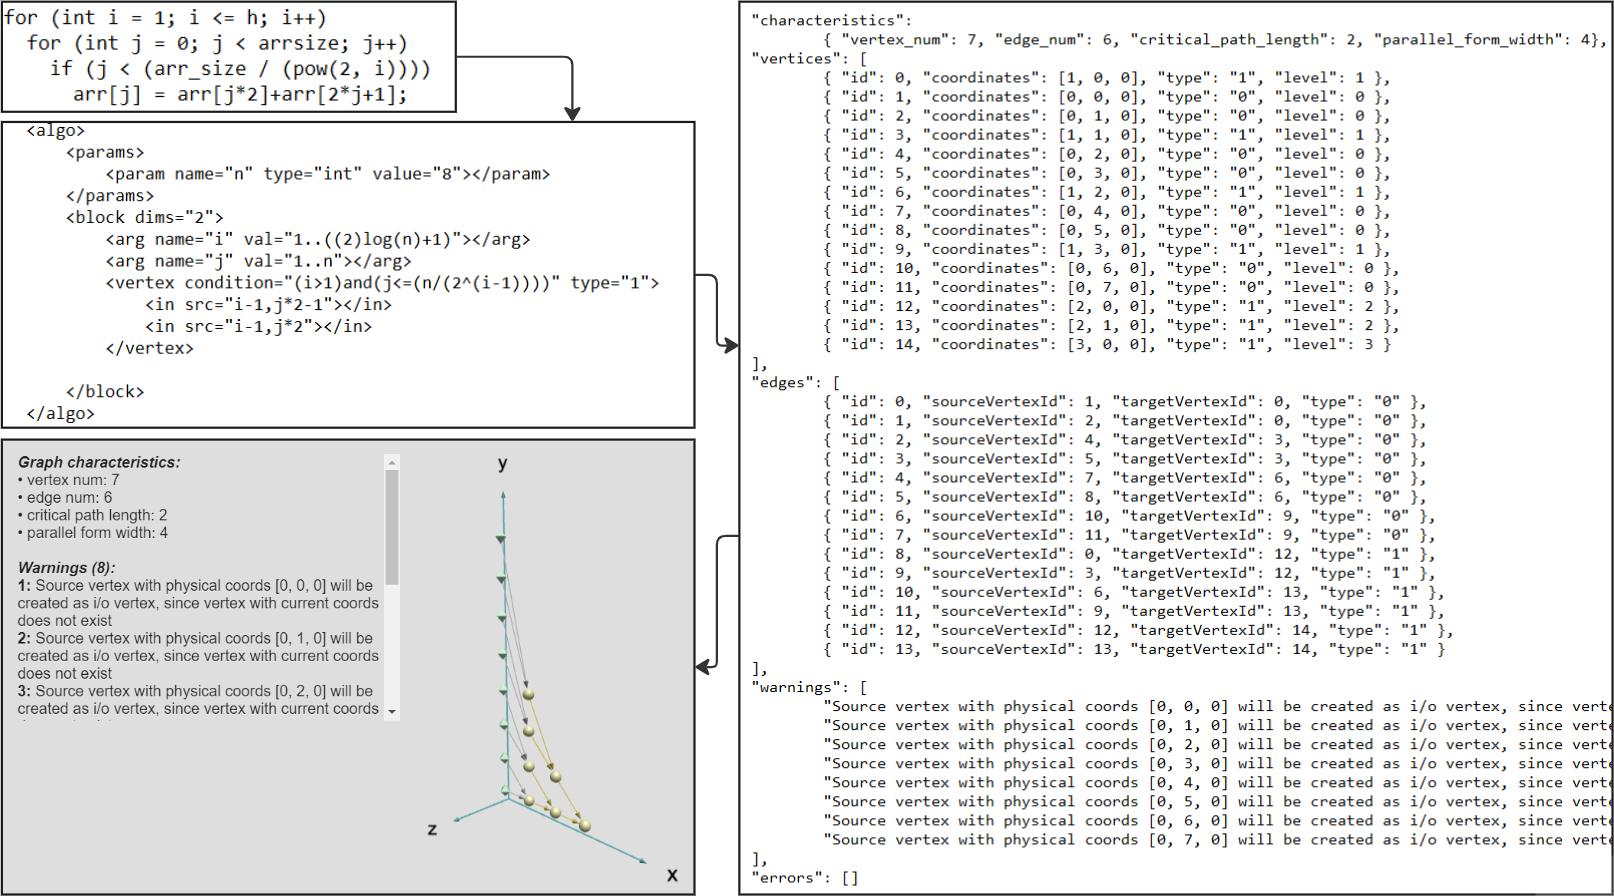
\includegraphics[height=6.78cm]{assets/algo_example.png}
\caption{Operation of the AlgoView system using the example of the algorithm ``Finding the sum of array elements by doubling'' for $n = 8$ from the implementation of the algorithm in the C language to the final visualization.}
\label{fig2}
\end{figure} % Описание Экспериментальной части
\section{Conclusion}

The article discusses the study of modern methods for developing a new version of the three-dimensional visualization system and interactive analysis of information graphs of AlgoView algorithms. The system in the described form is used for academic studies by master's students; we demonstrate its performance and usefulness for science and the study of information graph algorithms. The article shows the complete process of implementing the system and a description of the algorithms for its operation. The visualization system was tested on a large number of examples to identify problems and fix them. The system architecture is built taking into account future developments and additional modifications. Work on the project continues to expand the class of algorithms that the system can process and new ways of interactive graph analysis. % Заключение

%
% ---- Bibliography ----
%
\bibliographystyle{spmpsci}
\begin{thebibliography}{}


% \bibitem {czaj}
% Czajkowski, K., Fitzgerald, S., Foster, I., Kesselman, C.: Grid information services
% for distributed resource sharing. In: Proceedings 10th IEEE International Symposium
% on High Performance Distributed Computing, pp. 181--184. IEEE, New York (2001).
% \doi{10.1109/HPDC.2001.945188}


\bibitem {m1}
V.V. Voevodin, Vl.V. Voevodin. Parallel computing. St. Petersburg: BHV-Petersburg, 2002. 608 p. ISBN 5-94157-160-7. \url{https://www.studmed.ru/voevodin-vv-parallelnye-vychisleniya\_42cf5ce8568.html}
\bibitem {m2}
Volkov N.I. Algolang language documentation. \url{https://parallel.ru/sites/default/files/info/education/opisanie\_yazyka\_algolang.pdf}
\bibitem {m3}
Alexander S. Antonov, Alexey V. Frolov, Hiroaki Kobayashi, Igor N. Konshin, Alexey M. Teplov, Vadim V. Voevodin, Vladimir V. Voevodin. Parallel Processing Model for Cholesky Decomposition Algorithm in AlgoWiki Project // Supercomputing frontiers and innovations. — 2016. Volume 3. No. 3. - With. 61-70
\bibitem {m4}
AlgoWiki. Open encyclopedia of properties of algorithms. \url{https://algowiki-project.org}
\bibitem {m5}
AlgoWiki. Algorithm graph visualization standard. \url{https://algowiki-project.org}
\bibitem {m6}
Peter-Paul Koch. The Document Object Model: an Introduction. \url{https://www.digital-web.com/articles/the\_document\_object\_model/}
\bibitem {m7}
David Brownell. SAX2. - Gravenstein Highway North, Sebastopol: O’Reilly Media, 2002. - 240 p.
% \bibitem {m8}
% Difference between DOM vs SAX Parser in Java - XML Parsing in Java. \url{https://www.java67.com/2012/09/dom-vs-sax-parser-in-java-xml-parsing.html\#ixzz7xtkySKLe}
\bibitem {m9}
Sukumar Paul. How to Parse XML in C++. \url{https://linuxhint.com/parse\_xml\_in\_cpp/}
\bibitem {m10}
RapidXML library documentation. \url{https://rapidxml.sourceforge.net/}
\bibitem {m11}
PugiXML library documentation. \url{https://pugixml.org/}
\bibitem {m12}
TinyXML library documentation. \url{https://github.com/leethomason/tinyxml2}
% \bibitem {m13}
% PugiXML. Benchmarks. \url{https://pugixml.org/benchmark.html}
\bibitem {m14}
XSD: XML Data Binding for C++. \url{https://www.codesynthesis.com/products/xsd/}
\bibitem {m15}
Documentation of the RapidJSON library. \url{http://rapidjson.org/}
% \bibitem {m16}
% ExprTk library documentation. \url{https://github.com/ArashPartow/exprtk}
\bibitem {m17}
C++ Mathematical Expression Parsing And Evaluation Library. \url{http://www.partow.net/programming/exprtk/}
% \bibitem {m18}
% Joel Jones. Abstract Syntax Tree Implementation Idioms. \url{https://hillside.net/plop/plop2003/Papers/Jones-ImplementingASTs.pdf}
\bibitem {m19}
Documentation of the muParser library series. \url{https://beltoforion.de/en/muparserx/}
% \bibitem {m20}
% Muparser library documentation. \url{https://beltoforion.de/en/muparser/}
% \bibitem {m21}
% METL library documentation. \url{https://github.com/TillHeinzel/METL}
\bibitem {m22}
C++ Mathematical Expression Parser Benchmark. \url{https://github.com/ArashPartow/math-parser-benchmark-project}
\bibitem {m23}
S. Chaomei, Graph Drawing Algorithms, 2006. DOI:10.1007/1-84628-579-8\_3. \url{https://www.researchgate.net/publication/319727107\_Graph\_Drawing\_Algorithms}
\bibitem {m24}
S. Sim, Automatic Graph Drawing Algorithms. 1999. \url{https://www.researchgate.net/publication/2271614\_Automatic\_Graph\_Drawing\_Algorithms}
\bibitem {m25}
E.R. Gansner; E. Koutsofios; S.C. North; K.-P. Vo, A technique for drawing directed graphs, 1993. DOI: 10.1109/32.221135. Publisher: IEEE. \url{https://ieeexplore.ieee.org/document/221135}
\bibitem {m26}
V.N. Kasyanov, Methods and Tools for Visualization of Graphs and Graph Algorithms, 2021. INTERNATIONAL JOURNAL OF APPLIED MATHEMATICS AND INFORMATICS. DOI: 10.46300/91014.2021.15.13. \url{https://www.naun.org/main/UPress/ami/2021/a262013-013(2021).pdf}
\bibitem {m27}
M. Burch, G. Wallner, H. Wetering, F. Rooks, O. Morra, Visual Analysis of Graph Algorithm Dynamics, 2021. 14th International Symposium on Visual Information Communication and Interaction. DOI: 10.1145/3481549. \url{https://dl.acm.org/doi/10.1145/3481549.3481550}
\bibitem {m28}
Official website of the OpenGL library. \url{https://www.opengl.org}
\bibitem {m29}
Official website of the WebGL library. \url{https://www.khronos.org/webgl}
\bibitem {m30}
D. Carson, WebGL: Graphics and Animation, 2020. DOI:10.13140/RG.2.2.18538.95683. \url{https://www.researchgate.net/publication/344244517\_Research-Paper-WebGL}
\bibitem {m31}
M.J. Bian, H.H. Gao, J. Gao, Research and Application of Web3D Exhibition Based on WebGL and Html5, 2015. Conference: 2015 International Conference on Electrical, Automation and Mechanical Engineering. DOI:10.2991/eame-15.2015.220. \url{https://www.researchgate.net/publication/300618815\_Research\_and\_Application\_of\_Web3D\_Exhibition\_Based\_on\_WebGL\_and\_Html5}
\bibitem {m32}
Official website of the Three.js library. \url{https://threejs.org}
\bibitem {m33}
B. Danchilla, Three.js Framework, 2012. In book: Beginning WebGL for HTML5 (pp. 173-203). DOI:10.1007/978-1-4302-3997-0\_7. \url{https://www.researchgate.net/publication/302306483\_Threejs\_Framework}
\bibitem {m34}
Official website of the Babylon.js library. \url{https://www.babylonjs.com}
\bibitem {m35}
Official website of the VTK (Visualization Toolkit) library. \url{https://vtk.org}
\bibitem {m36}
Official website of the OpenSceneGraph library. \url{http://www.openscenegraph.com}
\bibitem {m37}
Official website of the DirectX API. \url{https://www.microsoft.com/ru-ru/download/details.aspx?id=35}
\bibitem {m38}
Official website of the Unity library. \url{https://unity.com}
\bibitem {m39}
Official website of the Blender platform. \url{https://www.blender.org}
\bibitem {m40} 
Official website of the Maya platform. \url{https://www.autodesk.com/products/maya/overview}
\bibitem {m41}
AlgoWiki. Glossary. \url{https://algowiki-project.org/ru/Glossary}
% \bibitem {m42}
% David Flanagan. JavaScript Pocket Reference, 3rd Edition. \url{https://www.oreilly.com/library/view/javascript-pocket-reference/9781449335977}
\bibitem {m43}
Official documentation of the OrbitControls module. \url{https://threejs.org/docs/\#examples/en/controls/OrbitControls}
\bibitem {m44}
GitHub repository of the dat.GUI module. \url{https://github.com/dataarts/dat.gui}
\bibitem {m45}
A.Majeed, I.Rauf, MVC Architecture: A Detailed Insight to the Modern Web Applications Development, 2018. \url{https://crimsonpublishers.com/prsp/pdf/PRSP.000505.pdf}
\bibitem {m46}
D.Pop, A.Samuel, Designing an MVC Model for Rapid Web Application Development, 2014. DOI:10.1016/j.proeng.2014.03.106. \url{https://www.researchgate.net/publication/275540078\_Designing\_an\_MVC\_Model\_for\_Rapid\_Web\_Application\_Development}



% \bibitem {m47}
% The official website of the Flask web framework. \url{https://flask.palletsprojects.com/en/3.0.x/\#}
% \bibitem {m48}
% Official website of the Docker platform. \url{https://www.docker.com/why-docker}
% \bibitem {m49}
% P. Gajer, M. Goodrich, S. Kobourov, A Fast Multi-Dimensional Algorithm for Drawing Large Graphs, 2000. \url{https://www2.cs.arizona.edu/~kobourov/grip\_paper.pdf}
% \bibitem {m50}
% M.Dodo, F.Andriamanampisoa, P.Torguet, J.Jessel, A new method to optimize the force-directed placement for 3D large graph drawing, 2007. Conference: Proceedings of the 5th International Conference on Computer Graphics, Virtual Reality, Visualization and Interaction. DOI: 10.1145/1294685.1294709. \url{https://www.researchgate.net/publication/220804553\_A\_new\_method\_to\_optimize\_the\_force-directed\_placement\_for\_3D\_large\_graph\_drawing}
% \bibitem {m51}
% GitHub repository for the MeshLine algorithm. \url{https://github.com/spite/THREE.MeshLine}
% \bibitem {m52}
% GitHub repository for the TextSprite algorithm. \url{https://github.com/SeregPie/THREE.TextSprite}
% \bibitem {m53}
% GitHub repository for the TextTexture algorithm. \url{https://github.com/SeregPie/THREE.TextTexture}

\end{thebibliography}
 % Литература

\end{document}
